\documentclass{article}

\usepackage[utf8]{inputenc}
\usepackage[danish]{babel}
\usepackage{float}
\usepackage{fancyhdr}
\usepackage{amsmath}
\usepackage{color}
\usepackage{listings}
\usepackage{graphicx}
\usepackage{pdfpages}
\usepackage{booktabs} 
\usepackage{listingsutf8}
%\usepackage{enumitem}
\usepackage[a4paper, top = 1in, bottom = 1in, left=1in,right=1in]{geometry}

\title{Exercise 6}
\author{Peter Heilbo Ratgen}
\date{\today}

\begin{document}
\maketitle
\section{Regression i R}
Vi laver regression på sammenhængen mellem alder og forbrug i baren.

\begin{figure}[h]
  \centering
  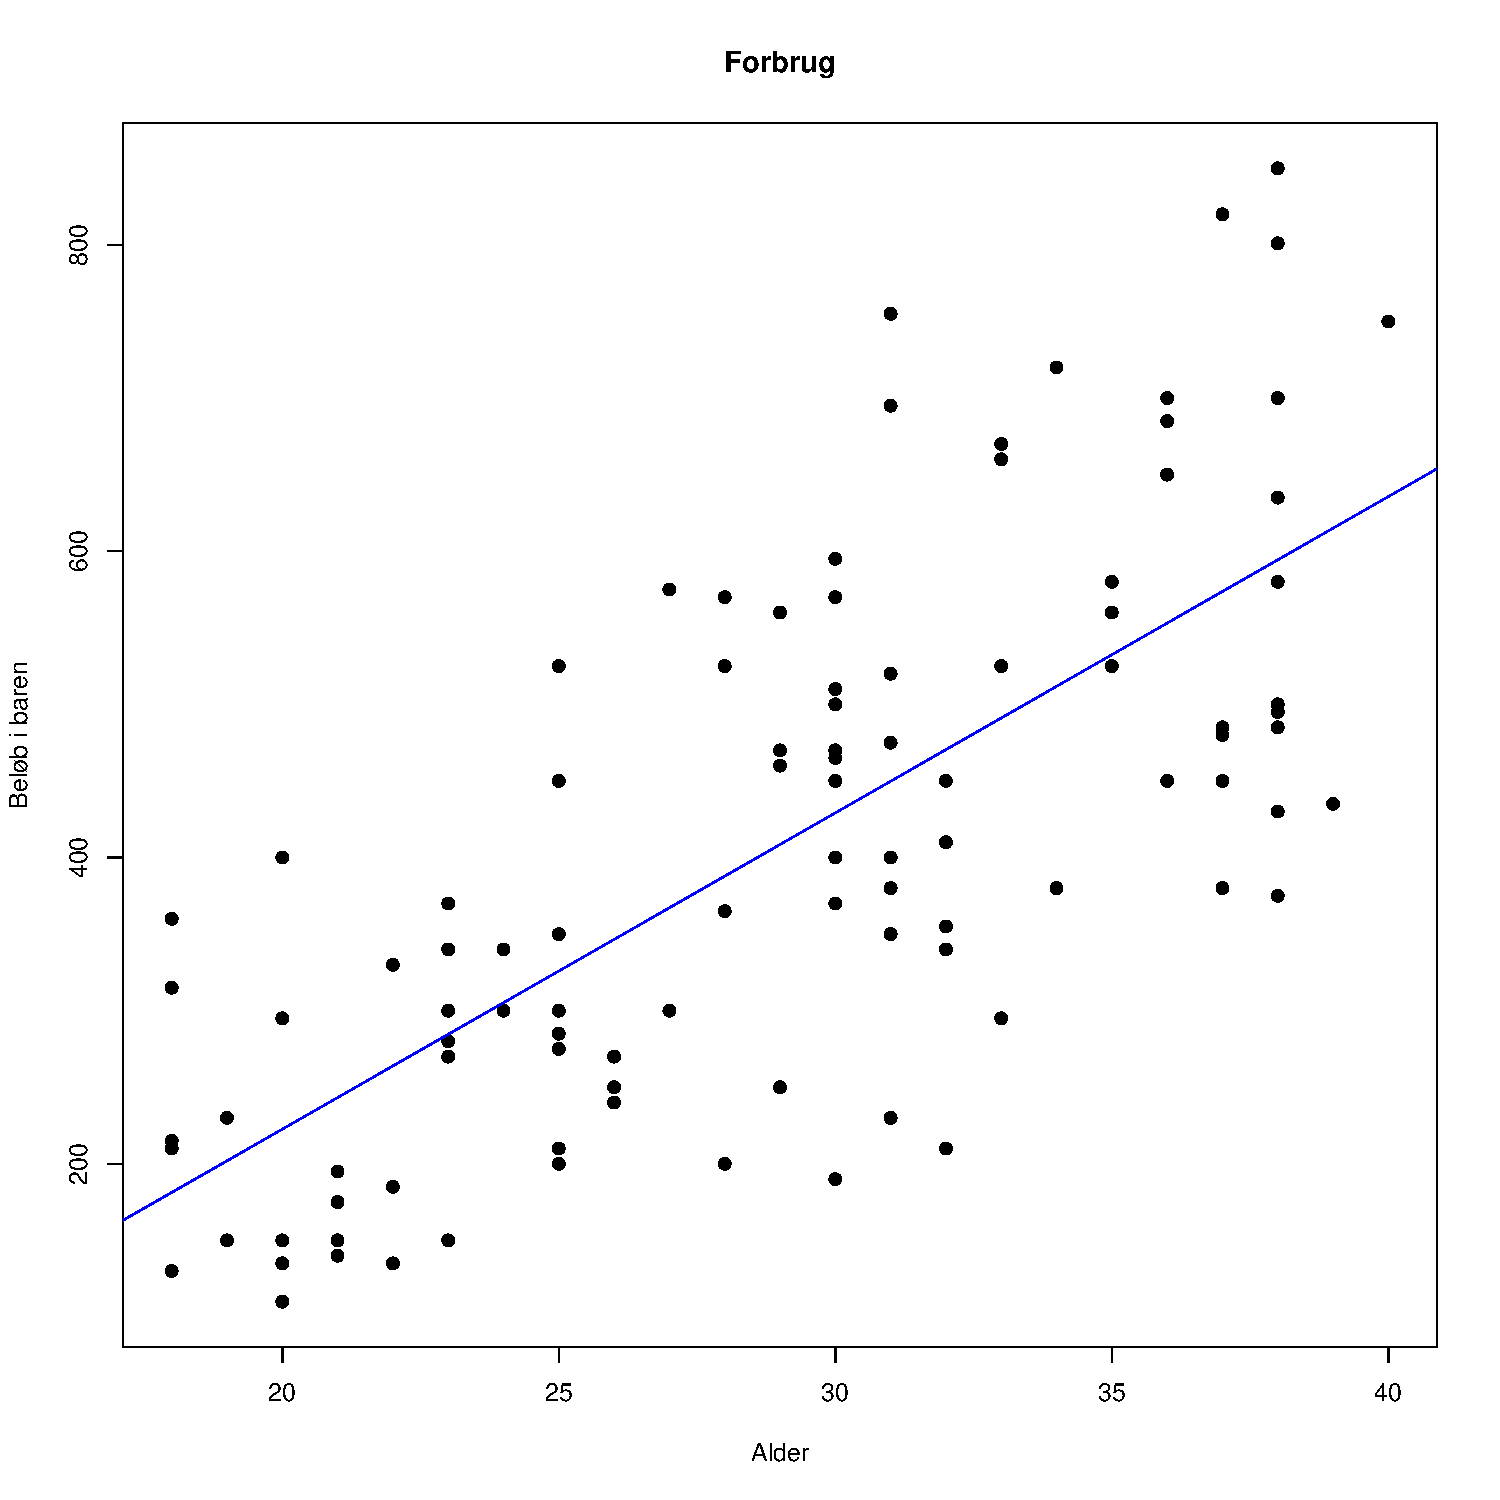
\includegraphics[width=0.65\textwidth]{../abline.pdf}
  \caption{caption}
\end{figure}

Vi laver en summering data:
\begin{lstlisting}[inputencoding=utf8/latin1,basicstyle=\ttfamily, language=R, keywordstyle=\color{blue}\bfseries, rulecolor=\color{black}]
@> summary(lmBar)

Call:
lm(formula = Beløb ~ Alder, data = bar)

Residuals:
    Min      1Q  Median      3Q     Max
-260.45  -94.37  -14.37   80.86  305.21

Coefficients:
            Estimate Std. Error t value Pr(>|t|)
(Intercept) -190.463     58.228  -3.271  0.00146 **
Alder         20.653      1.963  10.522  < 2e-16 ***
---
Signif. codes:  0 '***' 0.001 '**' 0.01 '*' 0.05 '.' 0.1 ' ' 1

Residual standard error: 125.7 on 103 degrees of freedom
Multiple R-squared:  0.5181,    Adjusted R-squared:  0.5134
F-statistic: 110.7 on 1 and 103 DF,  p-value: < 2.2e-16
\end{lstlisting}

Vi plotter residualerne for at se spredningen i forhold til regressions linjen.
Her ser vi at det er spredt jævnt.

\begin{figure}[h]
  \centering
  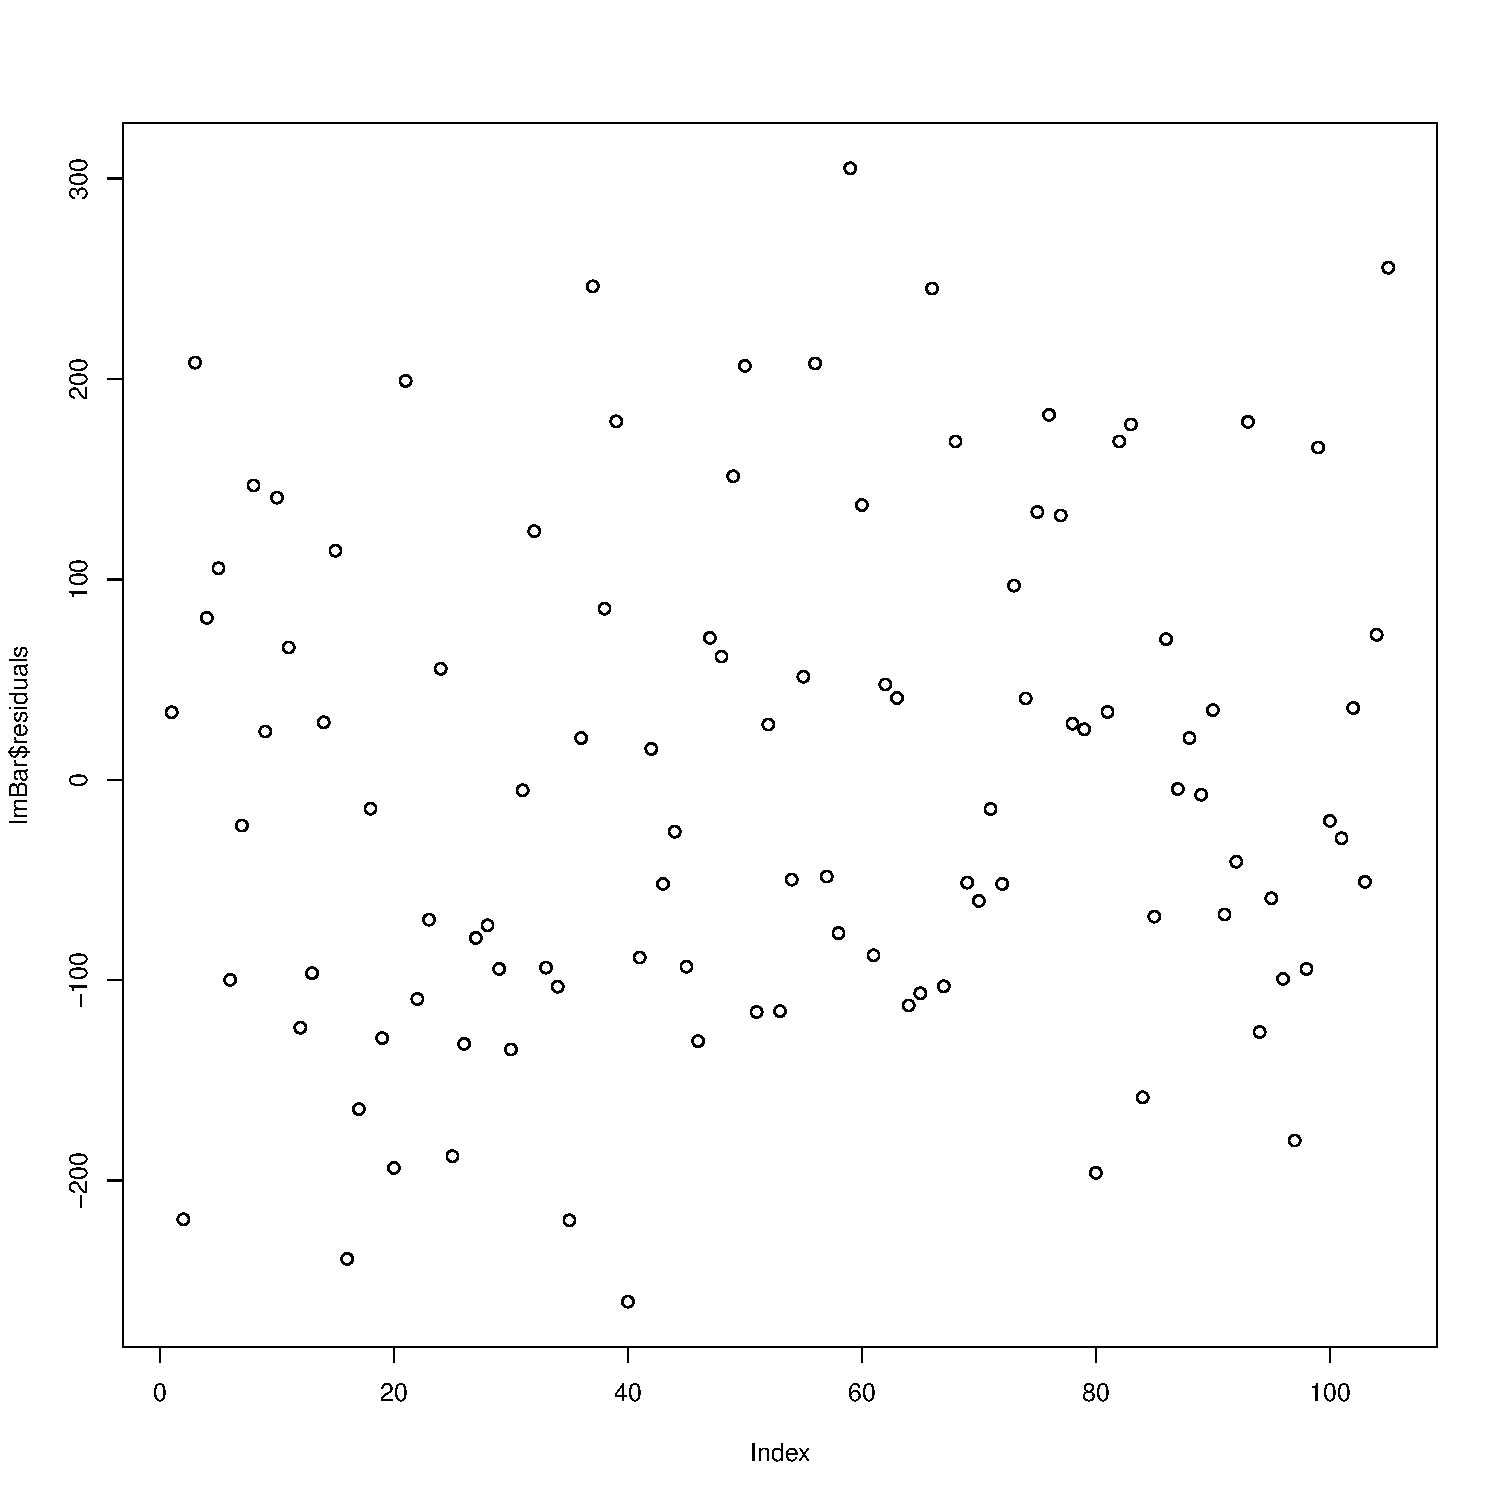
\includegraphics[width=0.65\textwidth]{../residualer.pdf}
  \caption{residualer}
\end{figure}


\section{Regressionskøleskab}

Vi skal undersøge sammenhængen mellem pris for køleskabe og deres volumen. Vi
kigger på et scatterplot over data.

\begin{figure}[H]
  \centering
  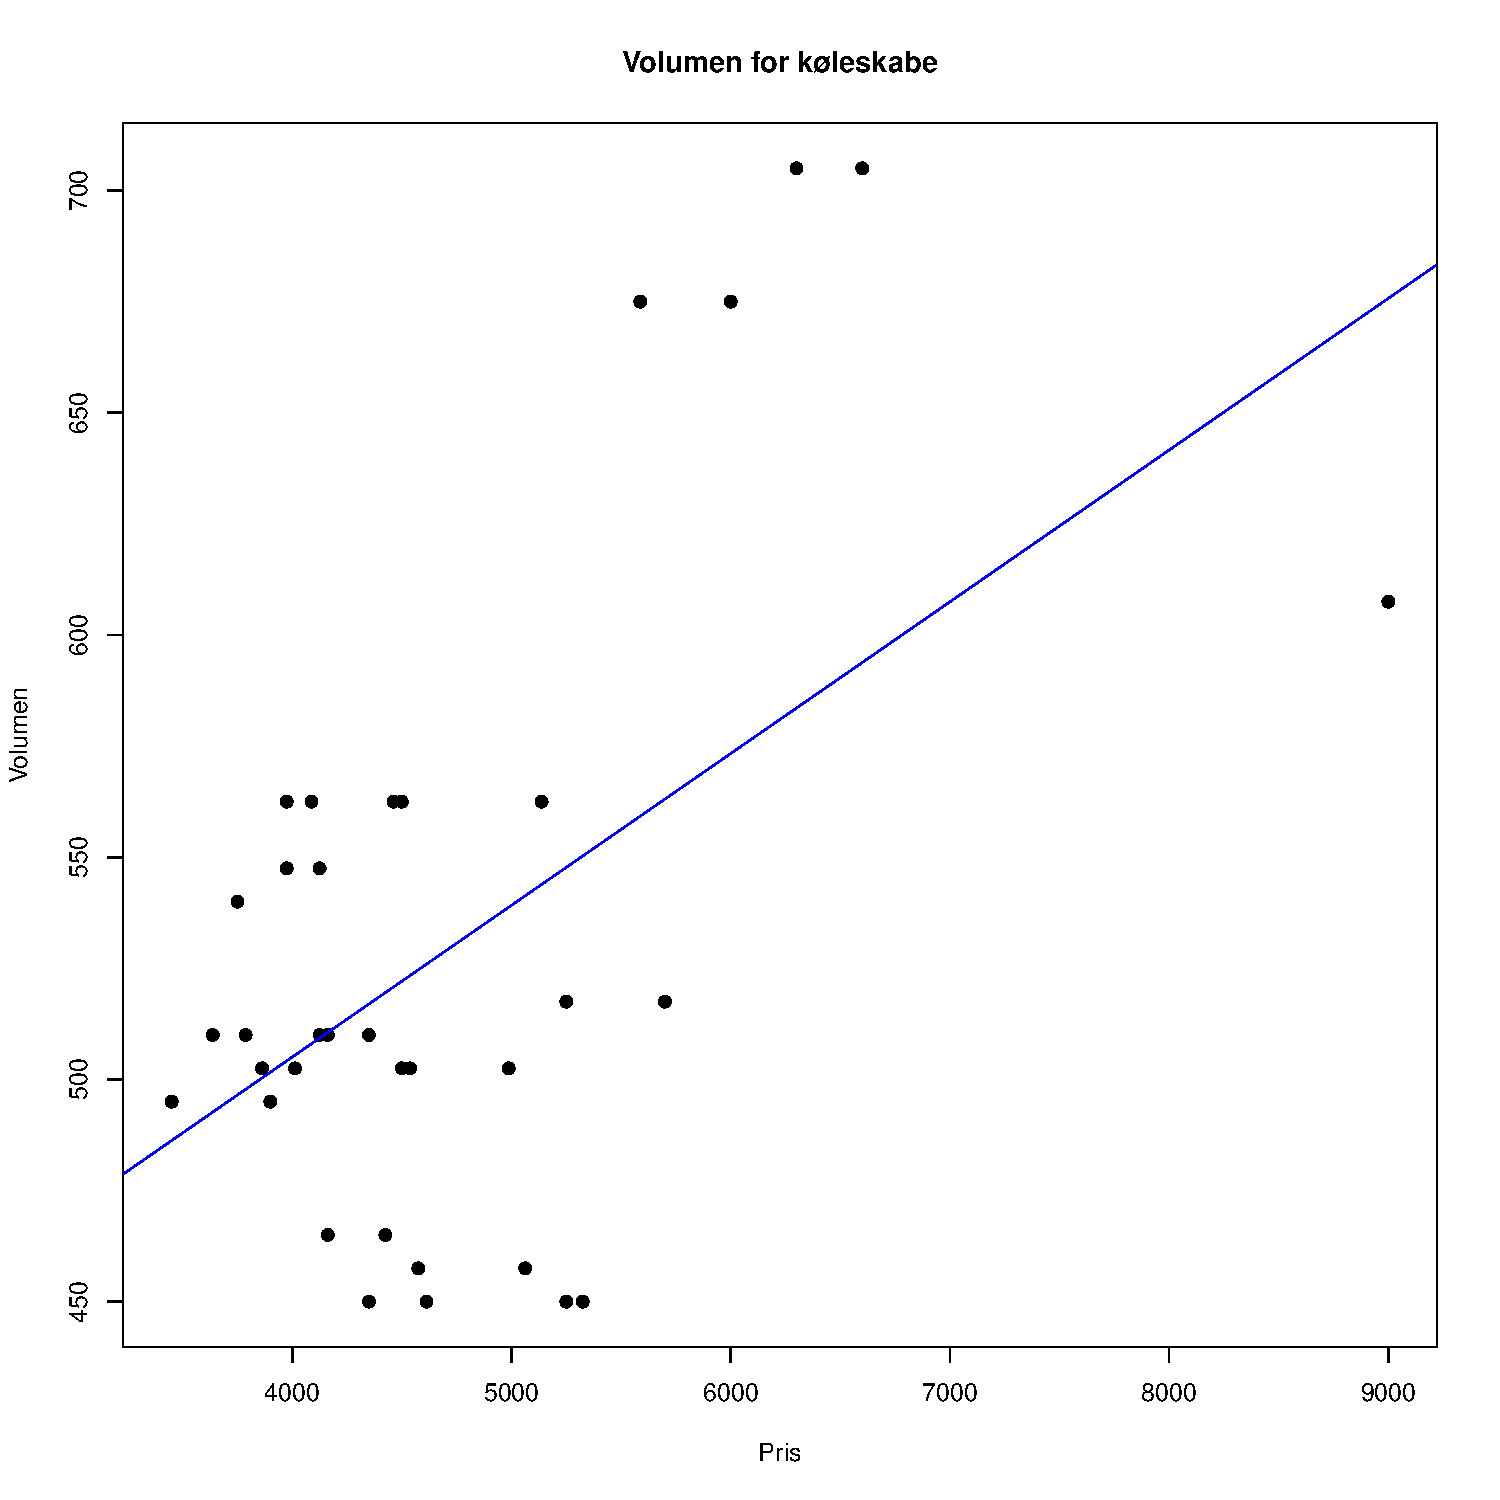
\includegraphics[width=0.65\textwidth]{../fridge_plot.pdf}
  \caption{caption}
\end{figure}

Det ligner at der kunne væren sammenhæng. Vi kigger på summeringen af
regressionen: 
\begin{lstlisting}[basicstyle=\ttfamily, language=R, keywordstyle=\color{blue}\bfseries, rulecolor=\color{black}]

@> summary(lmsum)

Call:
lm(formula = volumen ~ pris)

Residuals:
    Min      1Q  Median      3Q     Max
-100.27  -45.58   -0.58   40.40  121.44

Coefficients:
             Estimate Std. Error t value Pr(>|t|)
(Intercept) 3.685e+02  4.534e+01   8.127 1.43e-09 ***
pris        3.414e-02  9.425e-03   3.623 0.000915 ***
---
Signif. codes:  0 '***' 0.001 '**' 0.01 '*' 0.05 '.' 0.1 ' ' 1

Residual standard error: 59.29 on 35 degrees of freedom
  (25 observations deleted due to missingness)
Multiple R-squared:  0.2727,    Adjusted R-squared:  0.2519
F-statistic: 13.12 on 1 and 35 DF,  p-value: 0.0009155
\end{lstlisting}
Her kan vi se at der er en statistisk signifikant sammenhæng.
Ud fra det her kan vi også se at for hver 0.03413 i volumen for hver krone vi
bruger. Sammenhængen i modellen er ikke god, med omkring 0.25.

Vi plotter residualerne:
\begin{figure}[H]
  \centering
  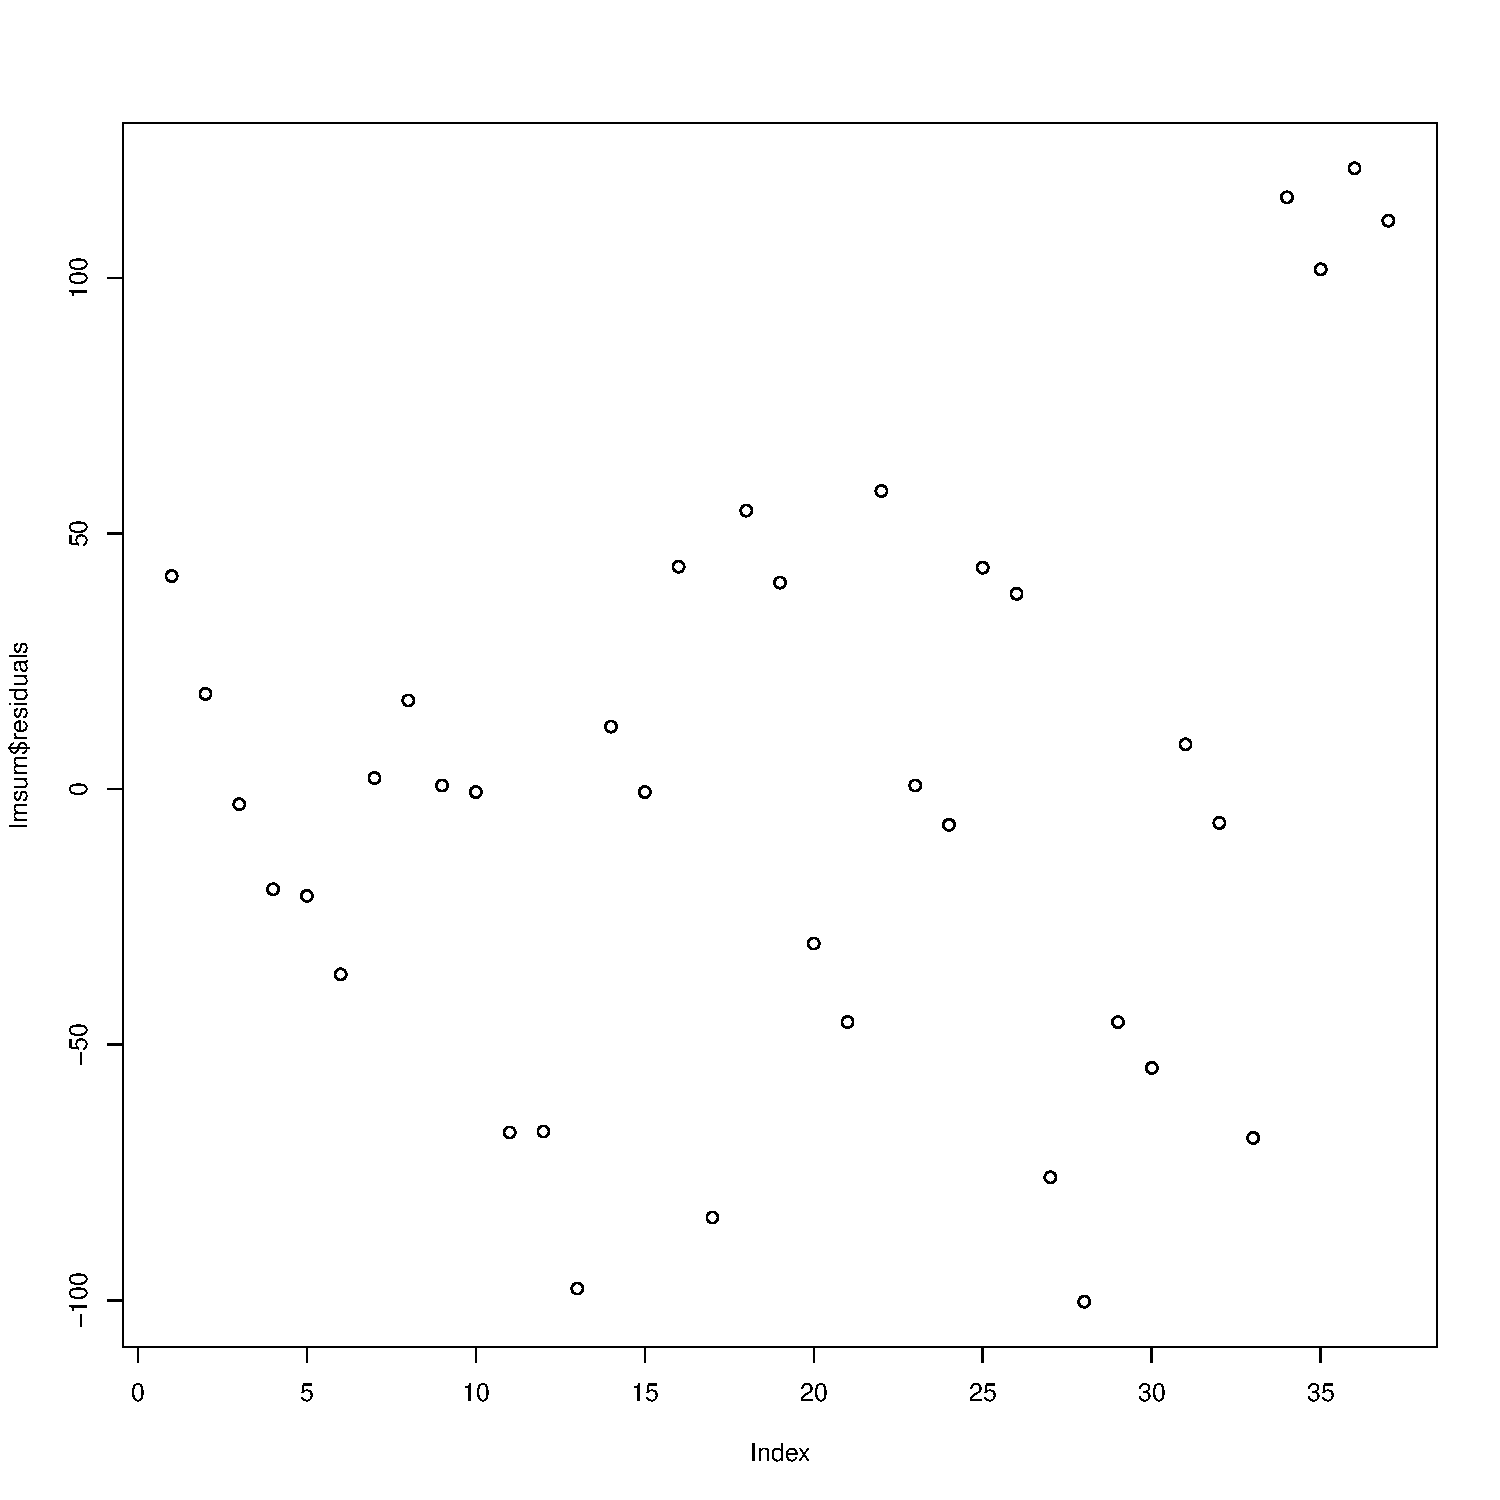
\includegraphics[width=0.685\textwidth]{../fridge_residuals.pdf}
  \caption{caption}
\end{figure}

Her residualerne spredt jævnt, modellen vurderes at være et godt fit.


\end{document}

